\documentclass[12pt, oneside]{article}
 
\usepackage{graphicx}
\graphicspath{ {./Pictures/} }
\usepackage{listings}
\usepackage{amssymb}
\usepackage{mathtools}
\usepackage[left=3cm,right=3cm,
    top=2cm,bottom=2cm]{geometry}

\usepackage{caption}
\usepackage[newfloat]{minted}
\usemintedstyle{borland}

\newenvironment{code}{\captionsetup{type=listing}}{}
\SetupFloatingEnvironment{listing}{name=Source Code}

\begin{document}
 
%titlepage
\thispagestyle{empty}
\begin{center}
\begin{minipage}{1\linewidth}
    \centering
%University logo

    
\includegraphics[width=0.3\linewidth]{logo-min.png}

    \vspace{2cm}
%Thesis title
    {\uppercase{\Large Report on the comparison of various integer multiplication algorithms\par}}
    \vspace{2cm}
%Author's name
    {\Large Anton Ivanov, under supervision of George Piatsky\par}
    \vspace{2cm}
%Degree
    {\Large DSBA, Group 191-1\par}
    \vspace{2cm}
%Date
    {\Large April 2020}
\end{minipage}
\end{center}
\clearpage


 \section{The Problem}
 The objective of this research is to estimate theoretical complexity of three different multiplication algorithms, namely \textbf{School-grade multiplication},
  \textbf{Divide and Conquer multiplication}, and \textbf{Karatsuba multiplication}, as well as to empirically prove or disprove possible hypotheses concerning the respective complexities of these algorithms
  
  \subsection {School-grade multiplication}
  The algorithm is based on the notions that are usually taught to people at school, this is where the name comes from. Basically, in order to multiply two integers of size $n$, one is ought to multiply each possible pair of integers (that is $n^2$ pairs) and then add this products to the resulting number, minding the positions to which add the products.\\ \textbf{Remark: }from now on term `problem size` will correspond to the length of both numbers that are going to be multiplied.
      \vspace{0.3cm}
  \\One of the possible implementations may look like this
  \begin{code}
\captionof{listing}{School-grade multiplication}
\begin{minted}[
frame=lines,
framesep=2mm,
baselinestretch=1.2,
fontsize=\footnotesize,
linenos
]{cpp}
 
Number SchoolMultiplicator::multiply(const Number &n1, const Number &n2) const
{
    std::string result(n1.size() + n2.size(), char(0));

    for (size_t i = 0; i < n1.size(); ++i)
    {
        int carry = 0;
        for (size_t j = 0; j < n2.size(); ++j)
        {
            result[i + j] += (n2.at(j) * n1.at(i) + carry);
            carry = result[i + j] / 10;
            result[i + j] %= 10;
        }
        result[i + n2.size()] = carry;
    }
    Number product = Number(std::move(result));

    return product;
}
  \end{minted}
    \end{code}
   Here numbers n1, n2 are stored as objects of class Number, that is based on std::string, where the element at index 0, char(last digit of the number). So number 123 is stored as [char(3), char(2), char(1)] 
         \vspace{0.3cm}
   \\
The basic intuition that we perform almost fixed number of operations $n^2$ times, suggest that $T(n) \in \Omega(n^2)$, if we denote number of seconds to needed to multiply two $n$-digit integers using this algorithm as $T(n)$. Moreover, our implementation also suggests that $T(n)$ is a quadratic function. Therefore, a \textbf{hypothesis} can be drawn.
      \vspace{0.5cm}
\\ \textbf{Hypothesis:} time complexity of \textbf{School-grade multiplication} $ =  \Theta(n^2)$. 

\subsection {Divide and Conquer multiplication}
  This recursive algorithm is based on the fact that $\displaystyle{\forall A \in \mathbb{N} \ \ \exists t \in \mathbb{N}: A = A_1 \cdot 10^t +  A_2} $ and therefore, product of two numbers A and B can be expressed as follows: 
  \[A B = (A_1\cdot10^t  + A_2)(B_1 \cdot 10^t +  B_2) = A_1B_1  \cdot 10^{2t} + (A_1B_2 + A_2B_1)\cdot 10^t + A_2B_2  \]
  This expression allows us to compute product of two $n$-digit numbers by instead computing 4 products of $\frac{n}{2}$-digit numbers as well as some additions.
     \begin{code}
\captionof{listing}{Divide and Conquer multiplication}

  \begin{minted}[
frame=lines,
framesep=2mm,
baselinestretch=1.2,
fontsize=\footnotesize,
linenos
]{cpp}
Number CaesarMultiplicator::multiply(const Number &n1, const Number &n2) const
{
    const size_t min_value = 1; // modify to optimize
    if (n1.size() <= min_value || n2.size() <= min_value)
    {
        std::unique_ptr<Multiplicator> fallback = std::make_unique<SchoolMultiplicator>();
        return fallback->multiply(n1, n2);
    }
    size_t m = std::min(n1.size(), n2.size()) / 2;

    //split numbers into two, one of which is of length m
    std::pair<Number, Number> a = n1.split(m);
    std::pair<Number, Number> b = n2.split(m);
    Number result;

    // A = A1 * t + A2
    // t = 10^m
    // AB = A1B1*t^2 + (A2B1 + A1B2)*t + A2B2 - 4 multiplications

    Number a1b1 = this->multiply(a.first, b.first);
    Number a2b2 = this->multiply(a.second, b.second);
    Number a1b2 = this->multiply(a.first, b.second);
    Number a2b1 = this->multiply(a.second, b.first);

    a2b1.shift(m);
    a1b2.shift(m);
    a1b1.shift(2 * m);

    return a1b1 + a2b1 + a1b2 + a2b2;
}

  \end{minted}
  \end{code}
  From this equality we can estimate the time complexity $T(n)$
  \[T(n) = 4T(n/2) + O(n)\]
  The formula can be `explained` as following: at each recursive call we have 4 subproblems, of size $n/2$, and addition can be done in linear time. Applying \textbf{Master Theorem} [Thomas H. Cormen. Charles E. Leiserson. Ronald L. Rivest. Clifford Stein 2009. Introduction to algorithms. Third edition, 94.] one receives $T(n) =\Theta(n^2)$
      \vspace{0.3cm}
\\ \textbf{Hypothesis:} time complexity of  \textbf{Divide and Conquer multiplication}$ =  \Theta(n^2))$
  
  \subsection {Karatsuba multiplication}
  
  This approach was proposed by Soviet mathematician Anatoly Karatsuba in 1960 and named after him. The algorithm is quite similar to \textbf{Divide and Conquer multiplication}, as it also recursive and bases on dividing main problem into many smaller subproblems, however here we have a different mathematical basis for it.
  \[A B =  A_1B_1  \cdot 10^{2t} + ((A_1 + A_2)(B_1 + B_2) - A1B1 + A_2B_2)\cdot 10^t + A_2B_2 \] 
  This expression allows us to compute product of two $n$-digit numbers by computing 3 products of $\frac{n}{2}$-digit numbers, instead of 4 as in \textbf{Divide and Conquer algorithm}, at a cost of performing more additions and substractions along the way.
    \begin{code}
\captionof{listing}{Karatsuba multiplication}

  \begin{minted}[
frame=lines,
framesep=2mm,
baselinestretch=1.2,
fontsize=\footnotesize,
linenos
]{cpp}
Number KaratsubaMultiplicator::multiply(const Number &n1, const Number &n2) const
{
    const size_t min_value = 1;// modify to optimize
    if (n1.size() <= min_value || n2.size() <= min_value)
    {
        std::unique_ptr<Multiplicator> fallback = std::make_unique<SchoolMultiplicator>();
        return fallback->multiply(n1, n2);
    }

    size_t m = std::min(n1.size(), n2.size()) / 2;

    //split numbers into two, one of which is of length m
    std::pair<Number, Number> a = n1.split(m);
    std::pair<Number, Number> b = n2.split(m);

    // A = A1 * t + A2
    // t = 10^m
    // AB = A1B1*t^2 + ((A1 + A2)(B1 + B2) - A1B1 - A2B2)*t + A2B2  - 3 multiplications
    Number a1b1 = this->multiply(a.first, b.first);
    Number a2b2 = this->multiply(a.second, b.second);
    Number a1_a2b1_b2 = this->multiply(a.first + a.second, b.first + b.second);

    Number intermediate = a1_a2b1_b2 - a2b2 - a1b1;
    a1b1.shift(2 * m);
    intermediate.shift(m);

    return a1b1 + intermediate + a2b2;
}
  \end{minted}
  \end{code}
  \[T(n) = 3T(n/2) + O(n)\]
   An `explanation` is similar as well: at each recursive call we have 3 subproblems, of size $n/2$, while additions and substractions can be done in a linear time. Applying \textbf{Master Theorem} one receives $T(n) = O(n^{\log_23}) \approx O(n^{1.6})$
    \vspace{0.3cm}
\\ \textbf{Hypothesis:} time complexity of  \textbf{Karatsuba multiplication}$ =  \Theta(n^{\log_2 3})$



All these hypotheses are also supported by the materials of the ADS course [ADS course, Lecture 19, S. Shershakov, 2020]

\section{Conditions of the experiment}
\subsection{A little bit about the implementation}
 The algorithms were implemented using the C++ programming language, with use of an auxilary class Number and a class Experimentator that was used to test to efficiency of the given multiplication algorithms. 
 
 Later in this page, \textbf{Divide and Conquer} algorithm will be simply called `Caesar` to shorten quite a clumsy name.
 

  \begin{figure}[h]
\caption{The class diagram}
\centering
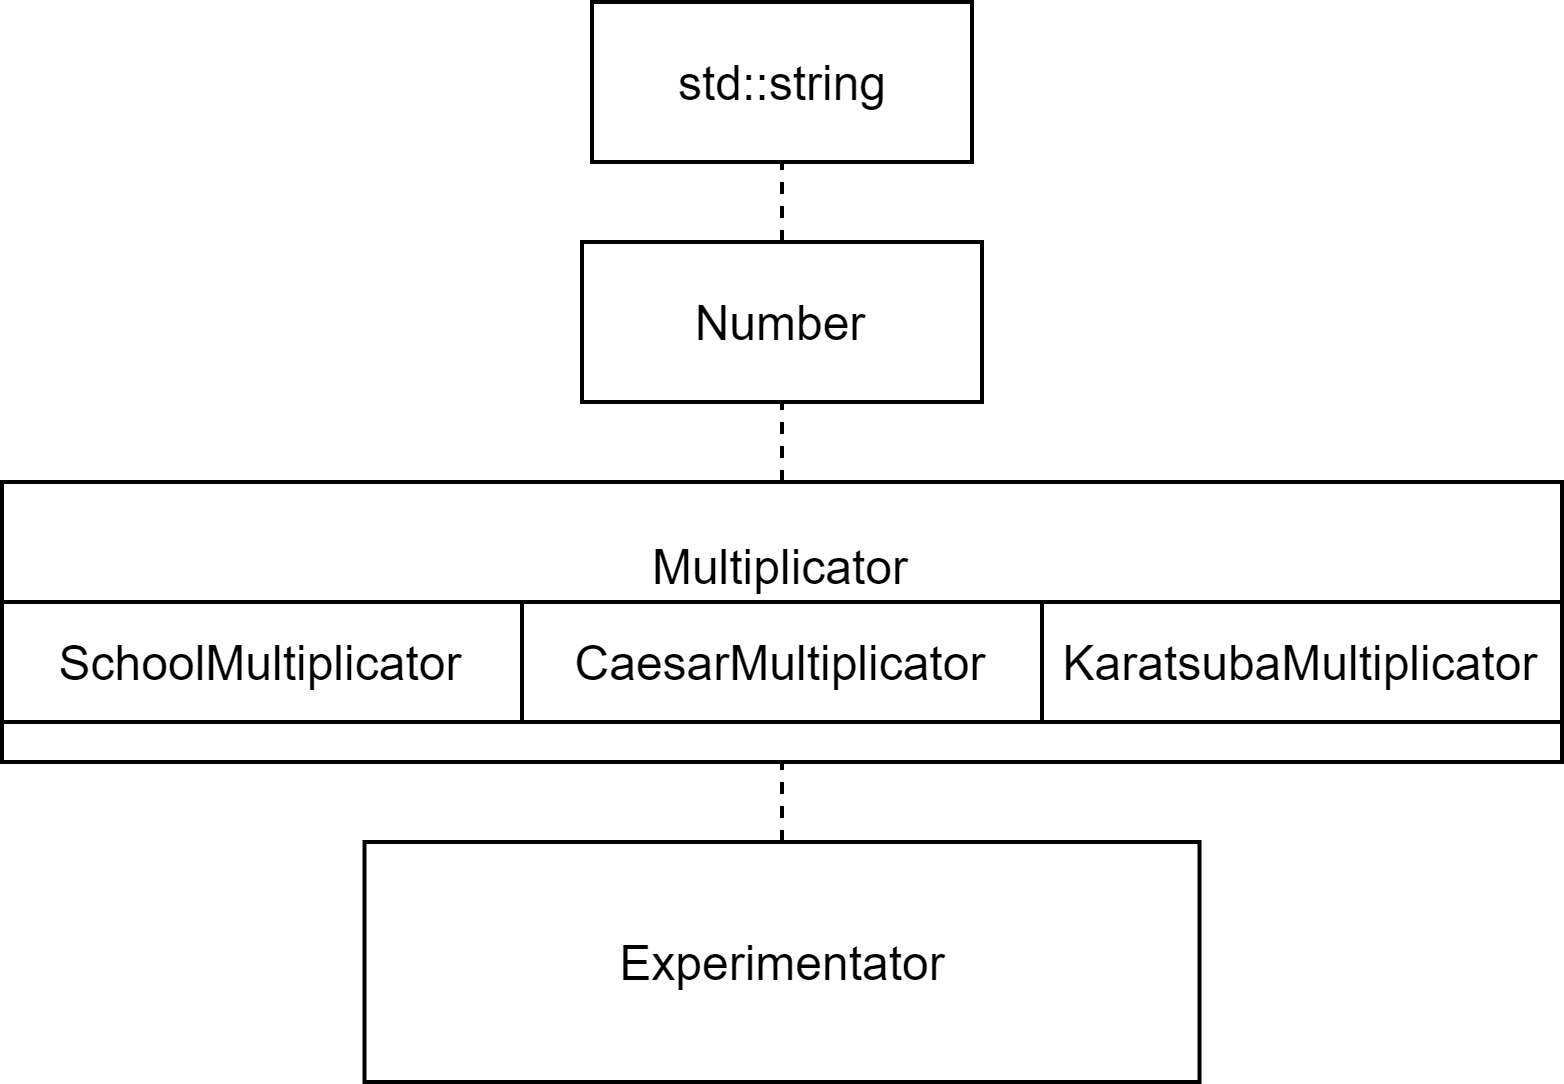
\includegraphics[width=1\textwidth]{Class Diagram}
\end{figure}
 Here notion of dashed lined should be read as `mainly depends on`, while inclusion of one area into another means that one is derived from another.
 All classes can be found at this link: 
 \underline{https://github.com/Olenek/dsba-ads2020-hw1}  
 

\subsection{General statements}
 Every algorithm has been tested using the same procedure consisting of four steps:
 \begin{enumerate}
 \item Generate a pair of two random $n$-digit numbers
 \item Run the tested algorithm on this pair of numbers, while measuring the running time, $k$ times, in order to reduce the random error. 
 \item Write the mean running time of the algorithm to the output csv file.
 \item Increment $n$ and redo steps 1, 2, and 3.
 \end{enumerate}
  For the experiment it was chosen to increment n in a pattern such that for all orders of numbers, n is changing in a way such that it iterates through an order in 10 steps. This procedure was executed with k = 3 with use of two additional methods: one to generate pseudorandom $n$-digit number and one to measure run-time of a function.

  \begin{code}
\captionof{listing}{Time measurement method}

  \begin{minted}[
frame=lines,
framesep=2mm,
baselinestretch=1.2,
fontsize=\footnotesize,
linenos
]{cpp}
double Experimentator::measure_time
  (const std::function<Number(const Number &, const Number &)> &f,
   const Number &n1,
   const Number &n2)
{
    auto start = std::chrono::high_resolution_clock::now();
    f(n1, n2);
    auto end = std::chrono::high_resolution_clock::now();
    auto duration = std::chrono::duration_cast<std::chrono::milliseconds>(end - start);

    return duration.count();
}

  \end{minted}
  \end{code}
  In this method, package $<$chrono$>$ is used to measure time in milliseconds between the beginning of the function execution and its end.
    \begin{code}
\captionof{listing}{Random number generator}


  \begin{minted}[
frame=lines,
framesep=2mm,
baselinestretch=1.2,
fontsize=\footnotesize,
linenos
]{cpp}
void Number::generate_random(size_t k, int time_seed)
{
    std::string randStr;
    std::srand(std::time(0) + time_seed);
    randStr.reserve(k);
    for (size_t i = 0; i < (k - 1); i++)
    {
        randStr.push_back(char(rand() % 10));
    }
    randStr.push_back(char((rand() % 9) + 1)); // adding the leading non-zero digit
    Number ans = Number(std::move(randStr));
    *this = ans;
}
  \end{minted}
  \end{code}
     In this function a random number is generated by creating a vector consisting of random digits, (with restriction on leading zero). Parameter 
   \textbf{time\_seed} ensures that \textbf{rand()} will be unpredictable from call to call.
   
   \begin{figure}[h]
\caption{The diagram of the testing process}
\centering
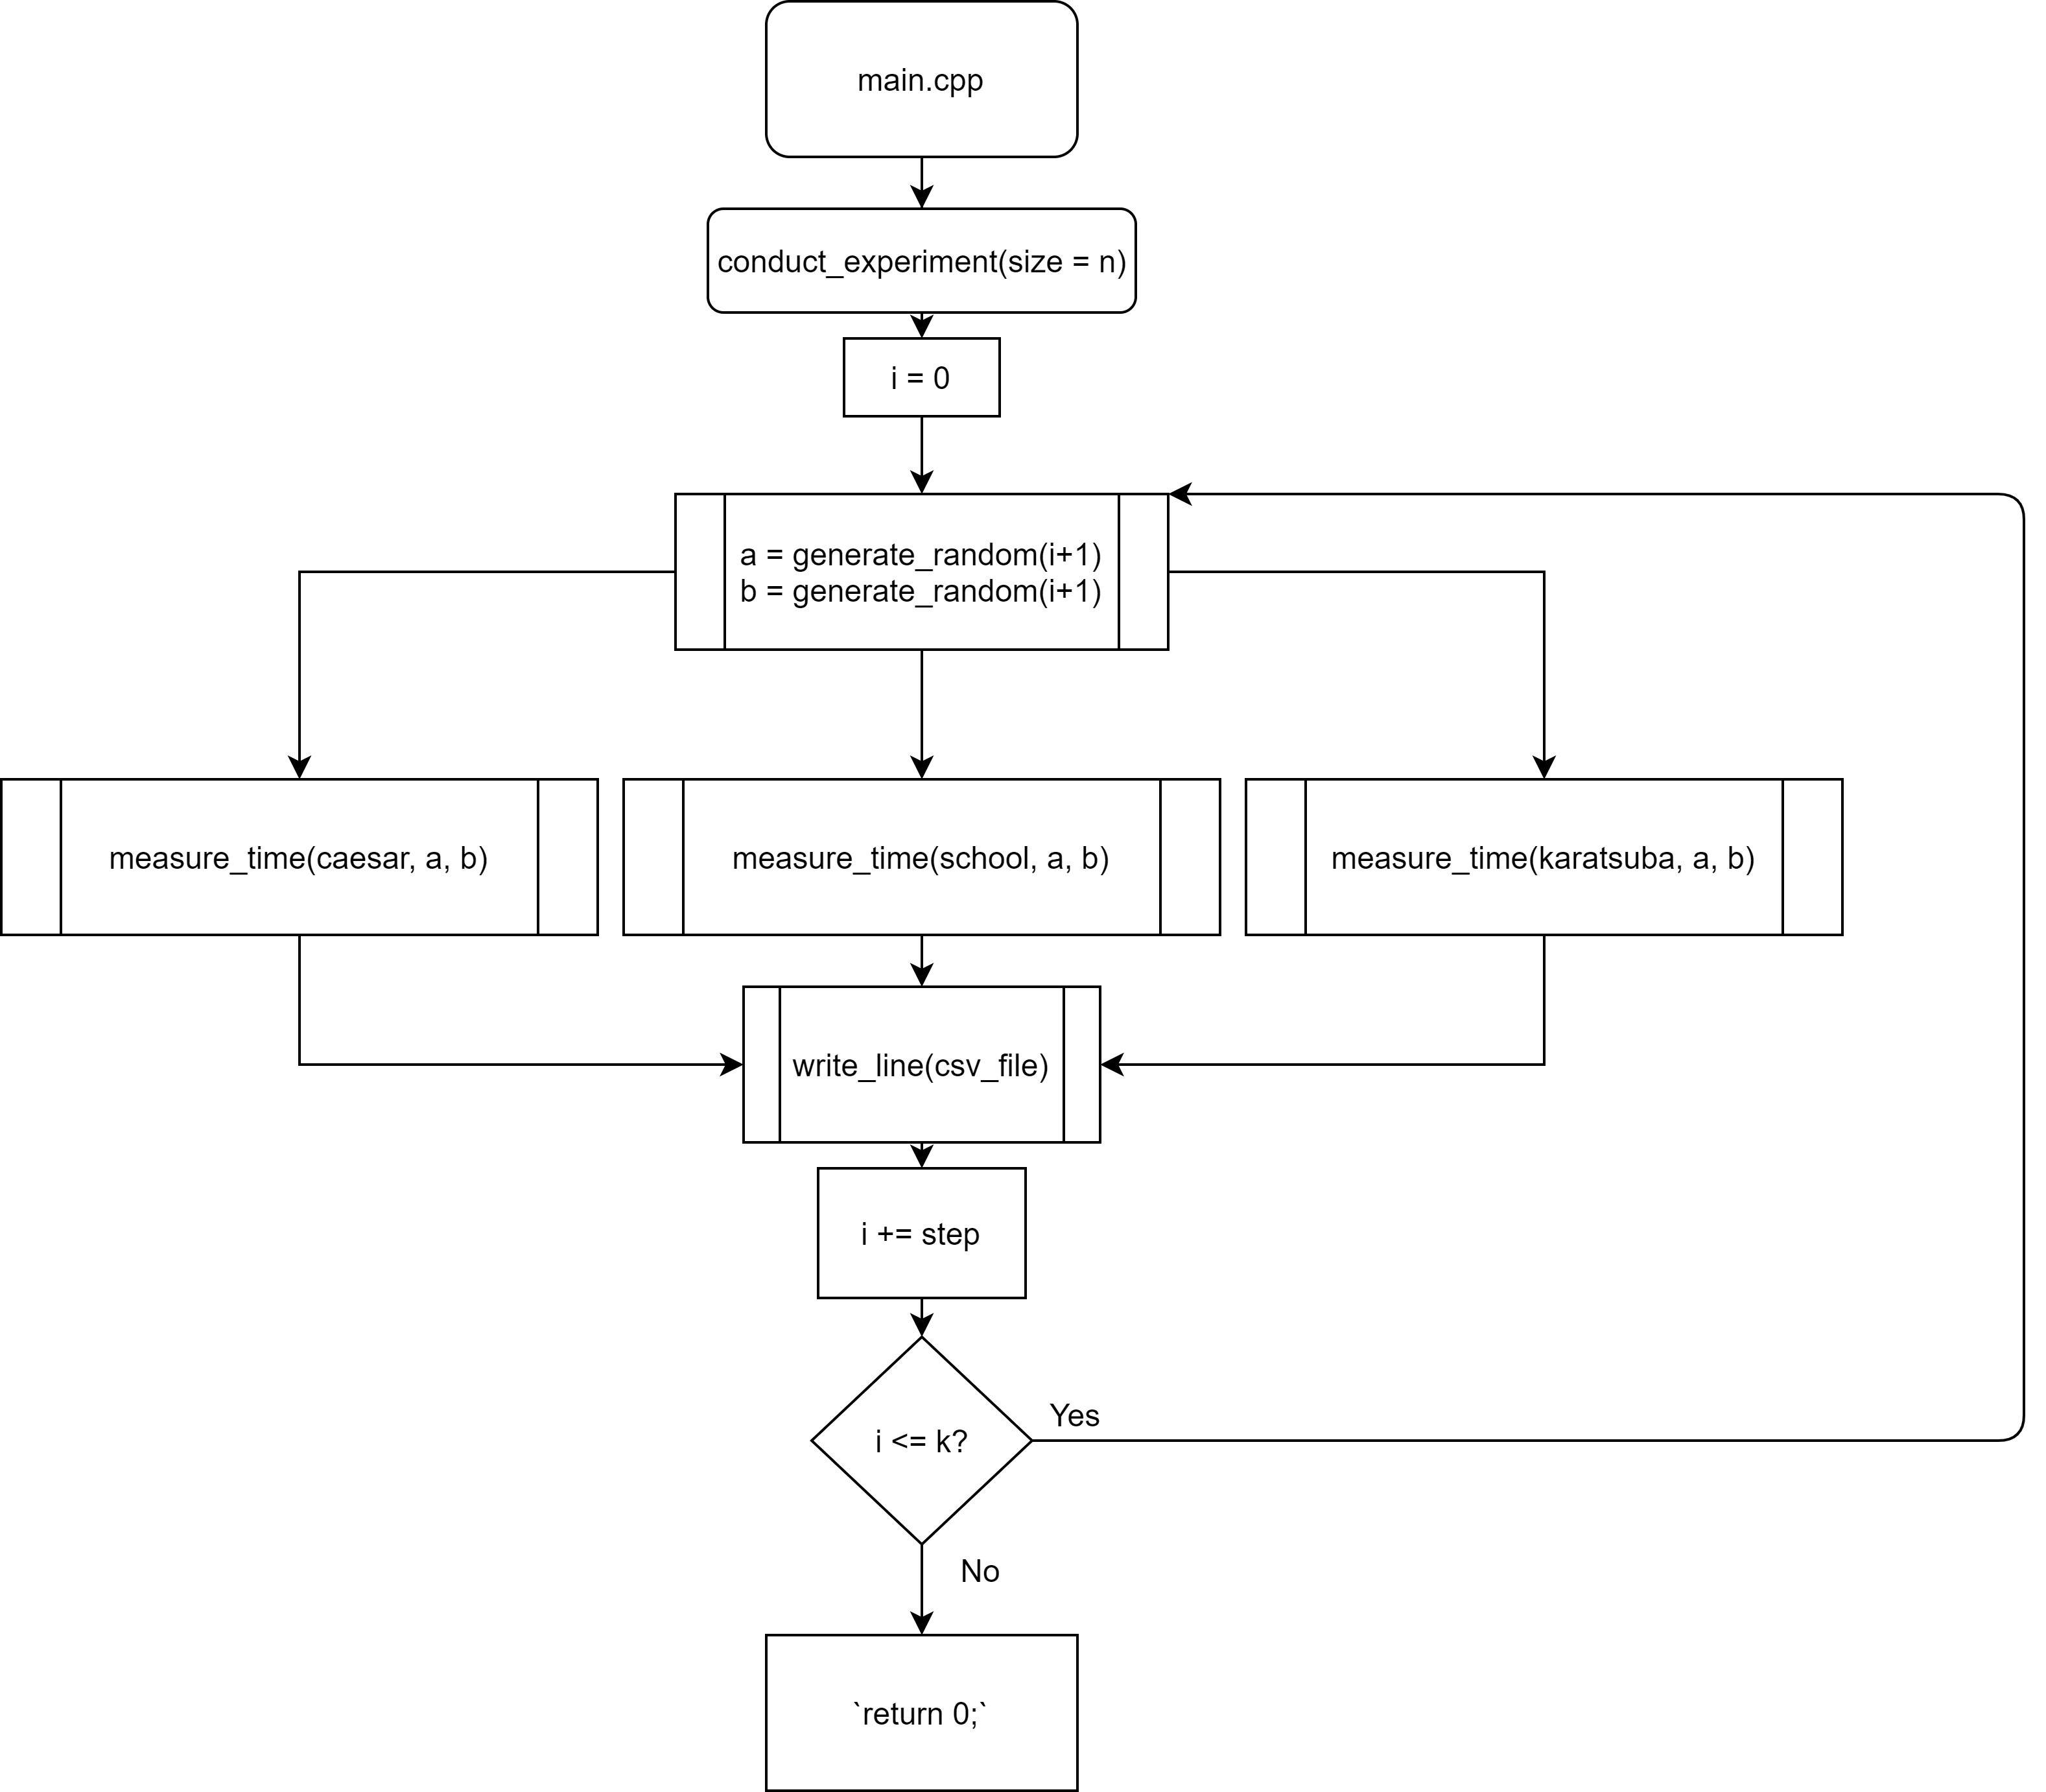
\includegraphics[width=1.15\textwidth]{ExperimentFlow}
\end{figure}
\textbf{Remark:} multiple measurements on the same problem size are not shown on the diagram to make it more readable.

\subsection{In brief}
Finally, it was decided to perform calculations of the running time of all three algorithms on problem sizes varying from 1 digit to 10001 digits with total of 73 data points. And then perform calculations of the running times of \textbf{Karatsuba} algorithm and \textbf{School-grade} algorithm on problem sizes varying from 1 digit to 100001 digits with total of 47 data points, in order to empyrically find when \textbf{Karatsuba} algorithm `beats` \textbf{School-grade} algorithm in terms of the running time.
\clearpage
\section{Processing of the results}

The graphs were made with use of Python and its module Pandas. All results of the experiment can be found in GitHub repository in directories `/result` and `/graphs`.

\begin{figure}[h]
\caption{Overall picture}
\centering
\includegraphics[width=1\textwidth]{Overview}
\end{figure}
The graph illustrates that \textbf{Divide and Conquer} (line `Caesar (ms)`) is always outperformed by its opponents. It can be explained as following: Divide and Conquer algorithm's depth of recursion is quite big. It is logarithmic and on each layer of recursion it calls itself 4 times, even when multiplying quite small numbers. One of the possible ways to optimize this algorithm is to allow it to multiply smaller numbers like \textbf{School-grade} multiplication does, while leaving multiplication of bigger numbers the same: calling itself 4 times with smaller problem size.  This topic will be addressed at the end of this article.

From this graph it is impossible to tell whether \textbf{Karatsuba} multiplication is more efficient or no. However another graph may help do this:


\begin{figure}[h]
\caption{Intersection point}
\centering
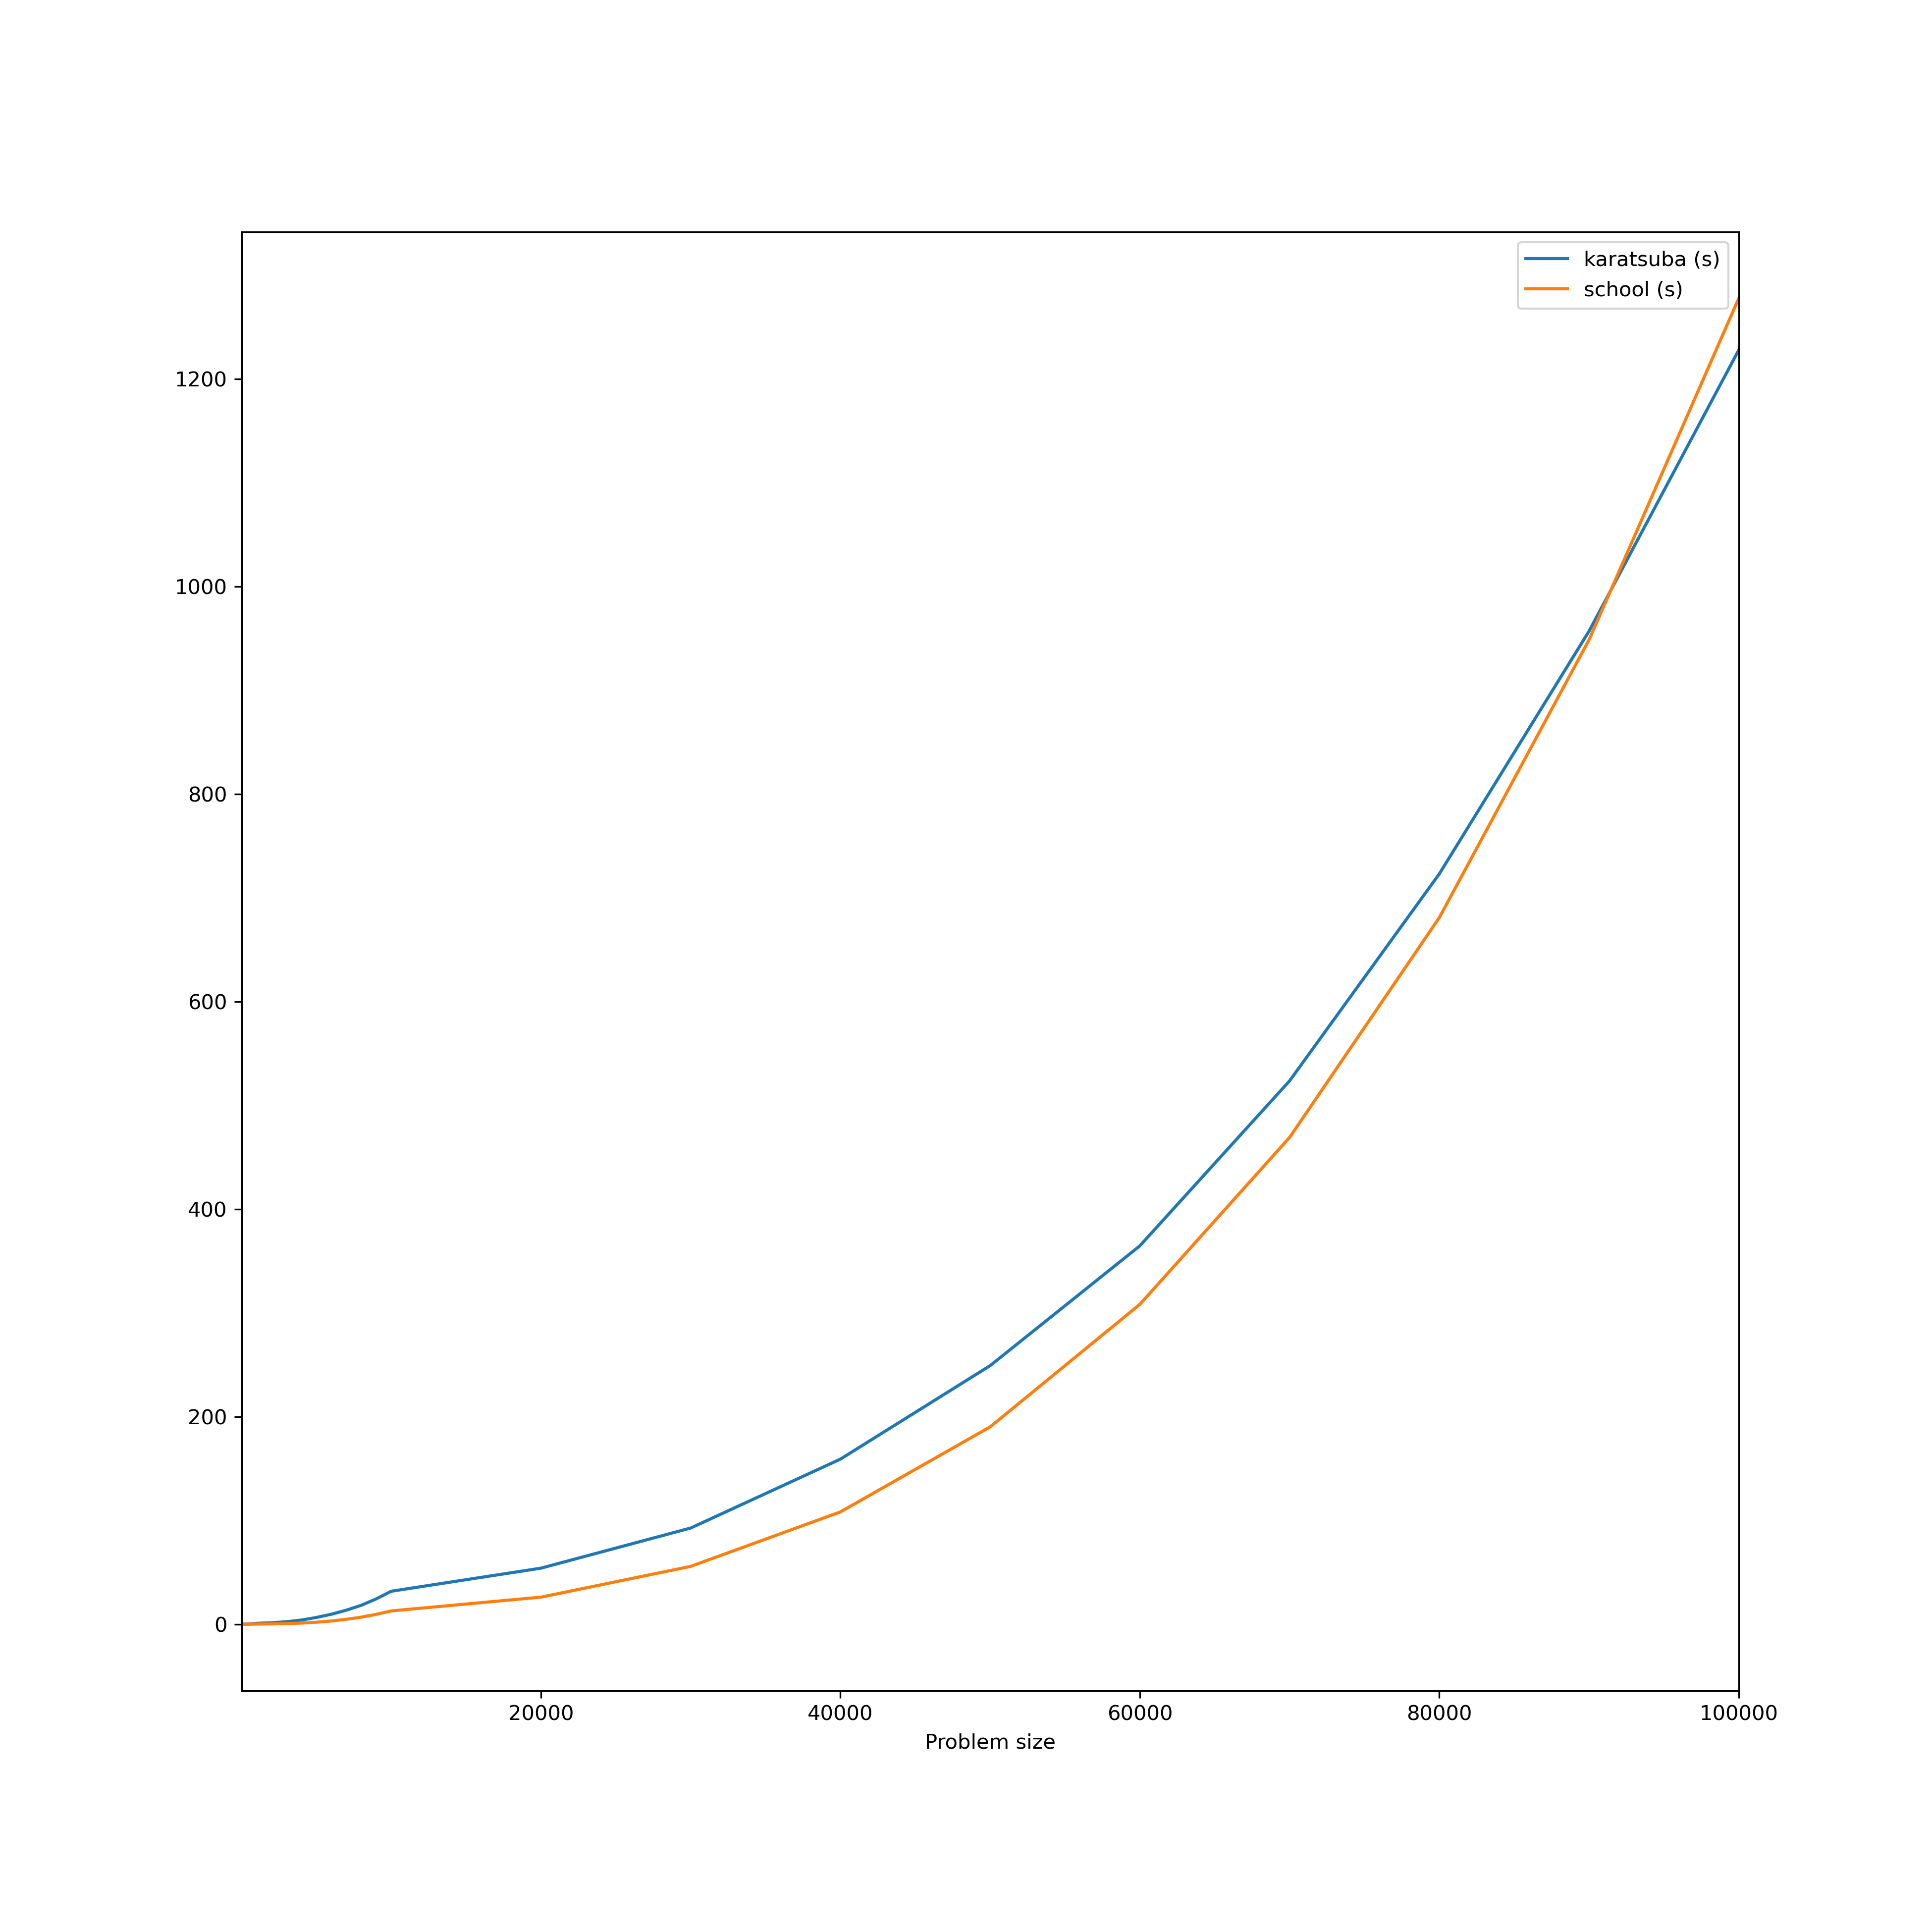
\includegraphics[width=1\textwidth]{intersection_square}
\end{figure}
\
This graph was made from file `intersection.csv` that was made with a different step-mechanism to make more frequent measurements. Details can be found in the repository.
  Here it can be seen that starting from around 90000 digits in a number, \textbf{Karatsuba} performs better than \textbf{School-grade}, however it does not mean that out hypotheses regarding time complexities are correct. We need another way to prove them.
\[f(n) \in \Theta(g(n)) \iff \exists k_1, k_2 \in \mathbb{R}_+:  \exists n_0: \forall n > n_0 \ \ k_1 g(n) \leq f(n) \leq k_2 g(n) \]  
The respective $k_1, k_2$ are represented in the graphs.
  \begin{figure}[h]
\caption{School-grade $\in \Theta(n^2)$}

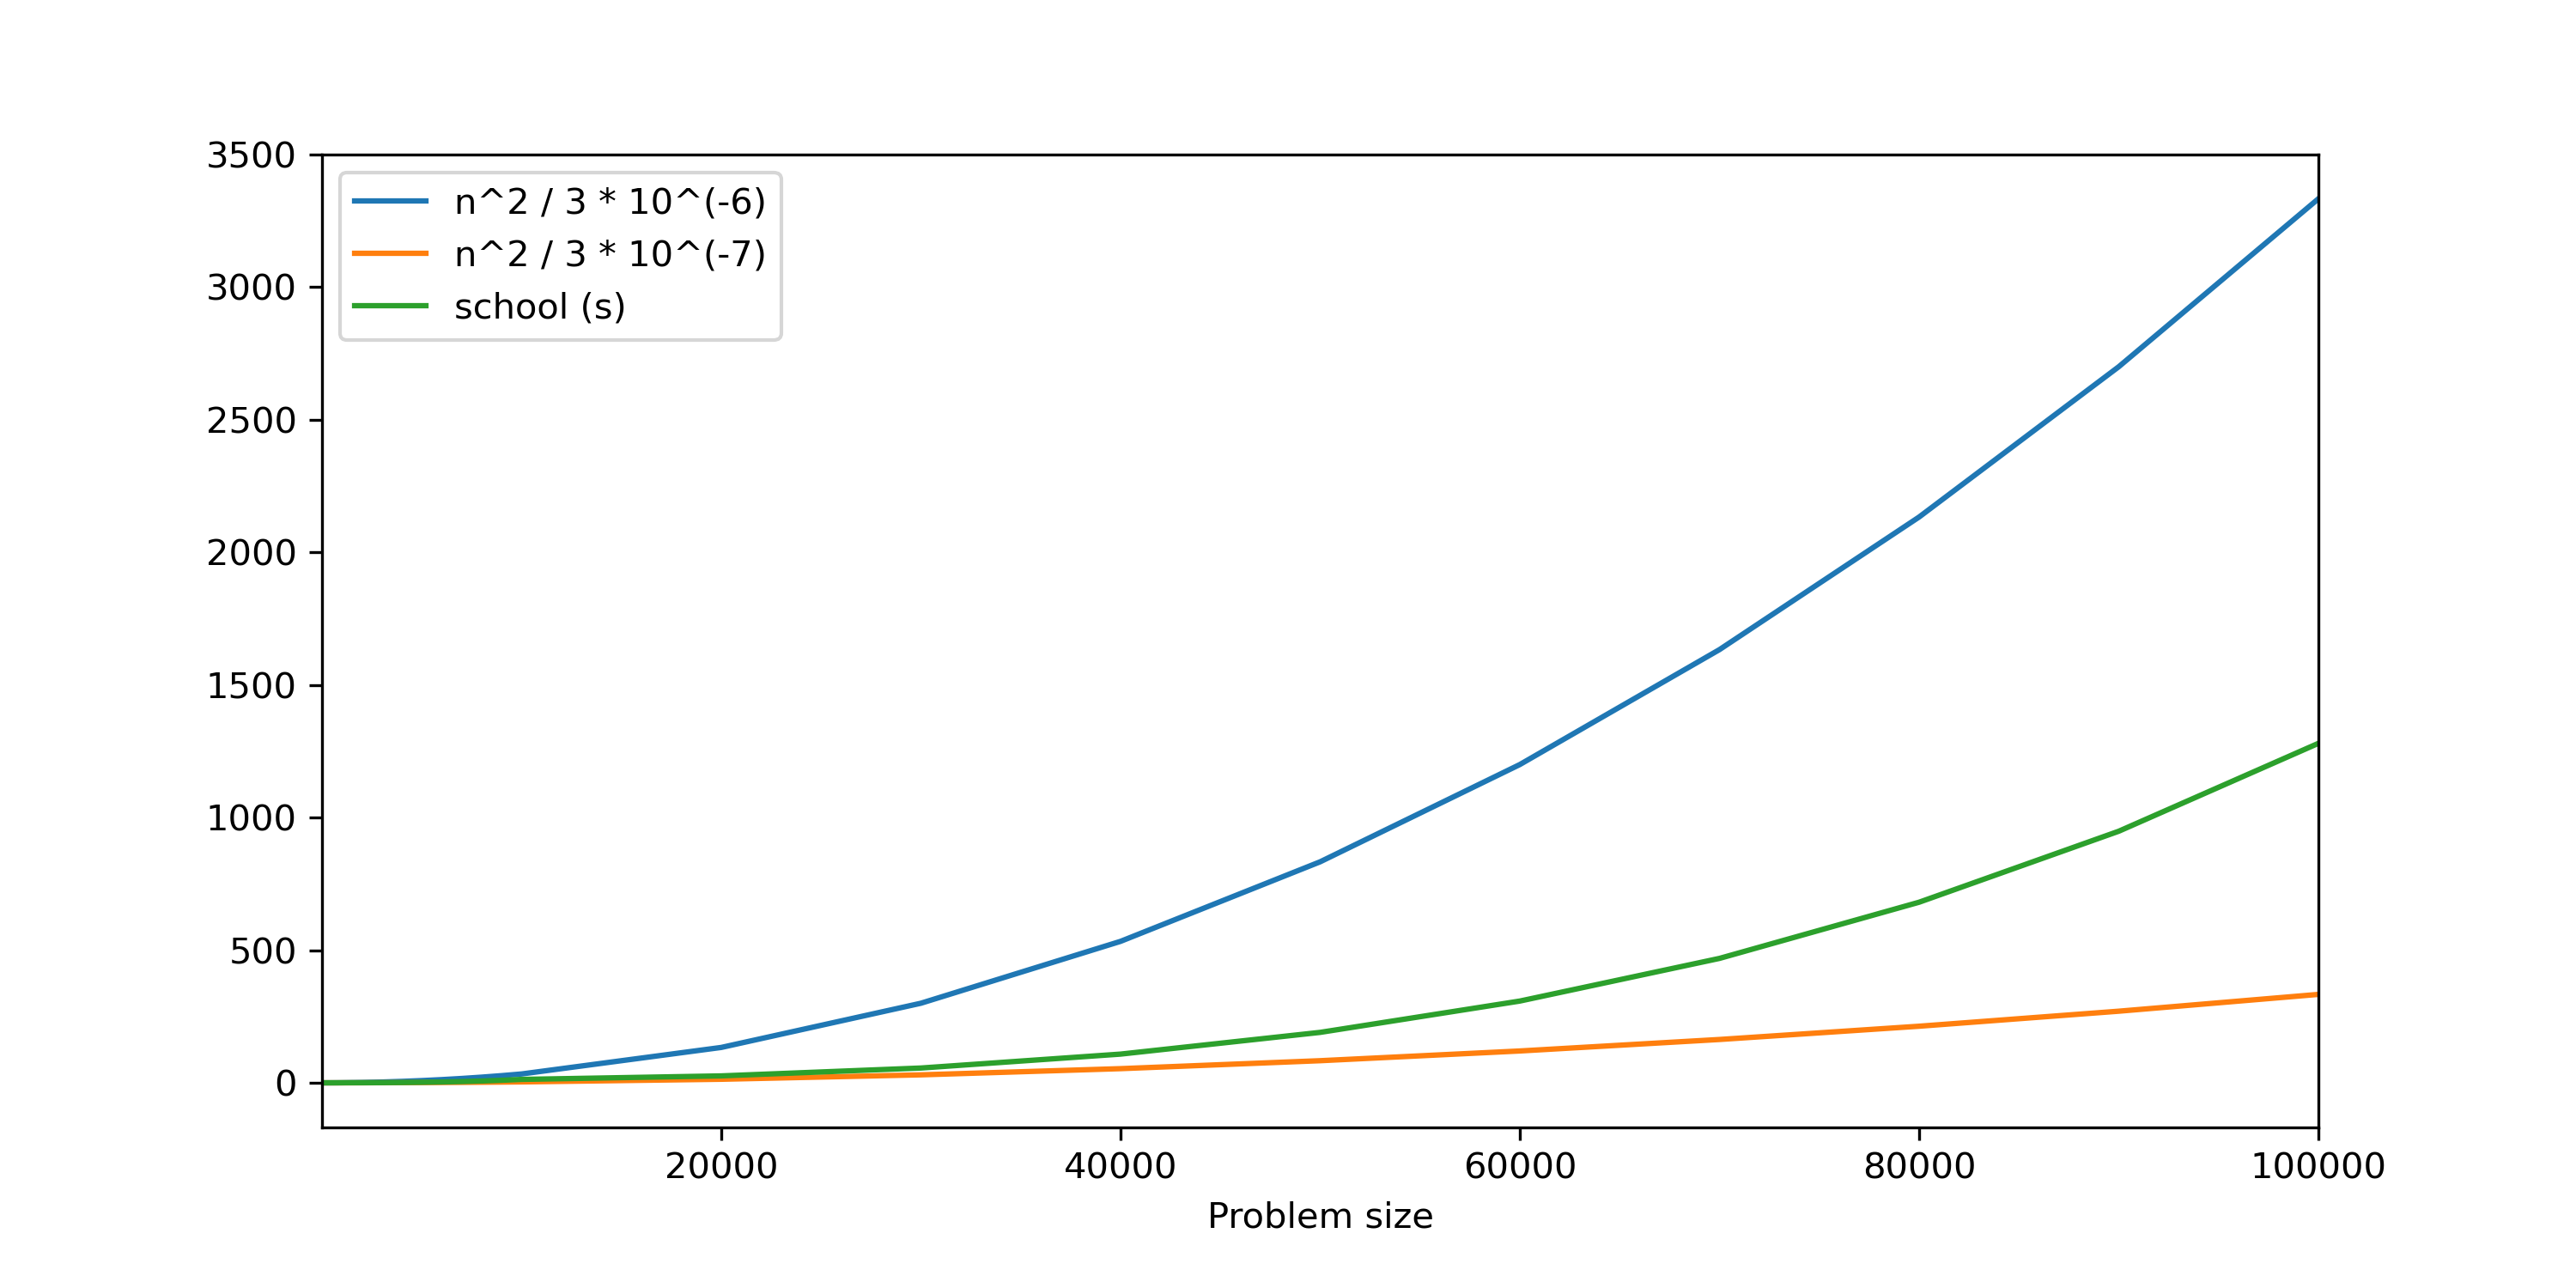
\includegraphics[width=1\textwidth]{O_school}
\end{figure}
\begin{figure}[h]
\caption{Karatsuba $\in \Theta (n^{\log_2 3})$}

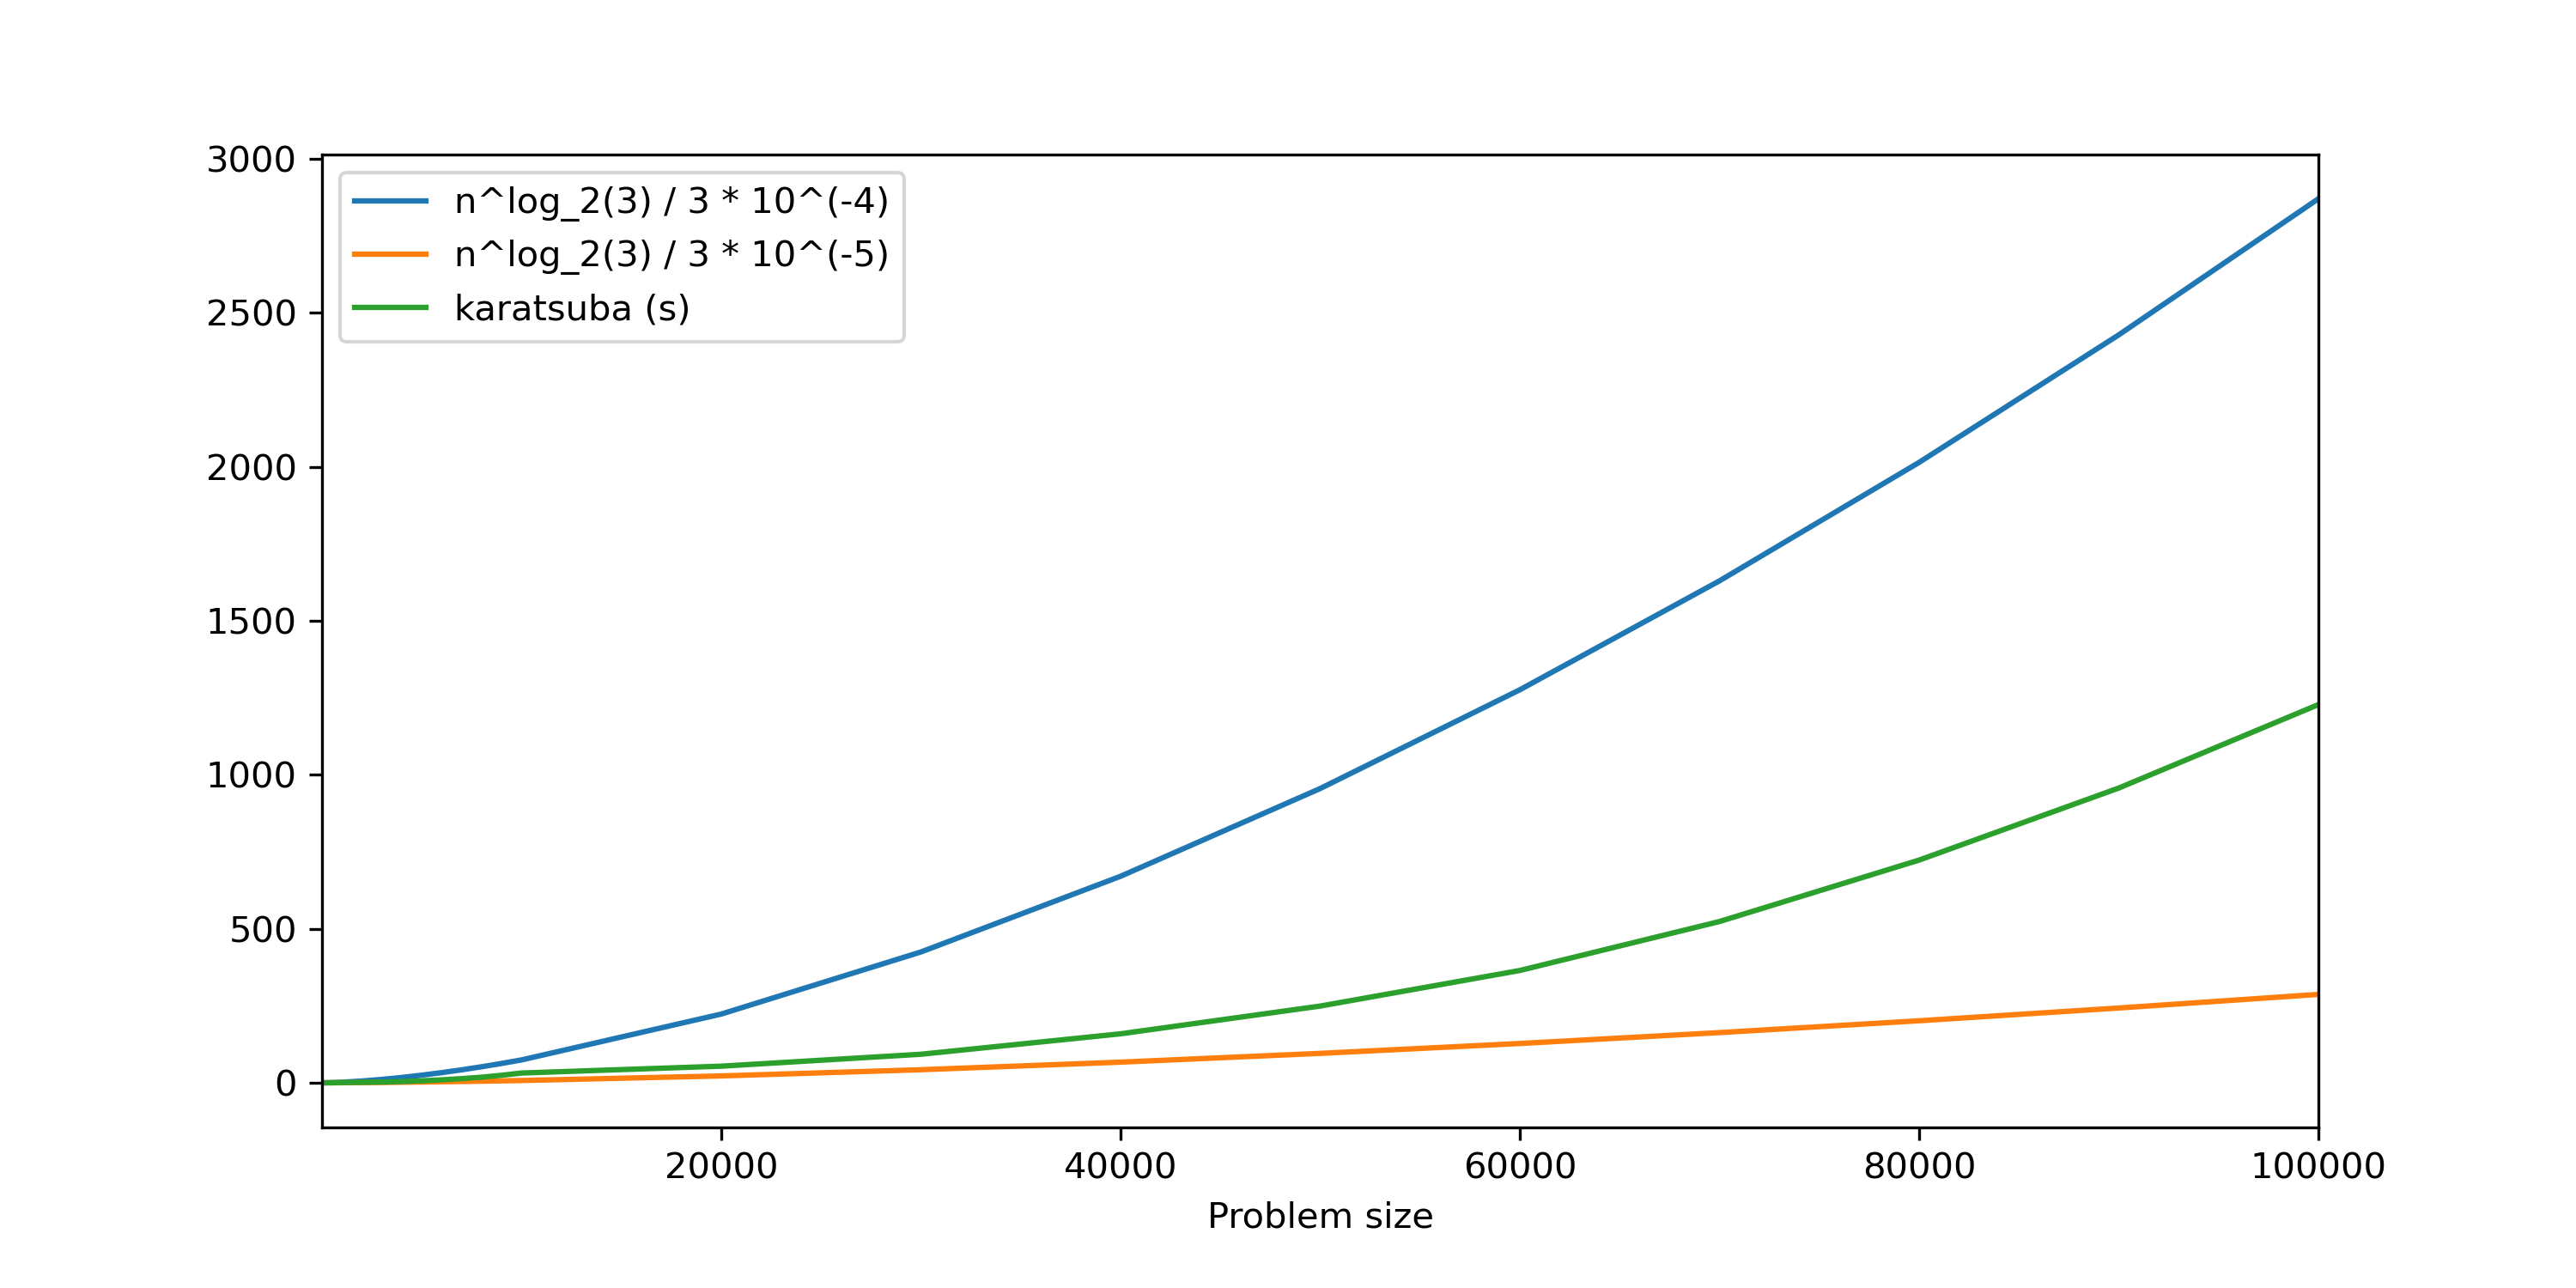
\includegraphics[width=1\textwidth]{O_karatsuba}
\end{figure}
\clearpage
\begin{figure}[t]
\caption{Divide and Conquer (Caesar) $\in \Theta(n^2)$}

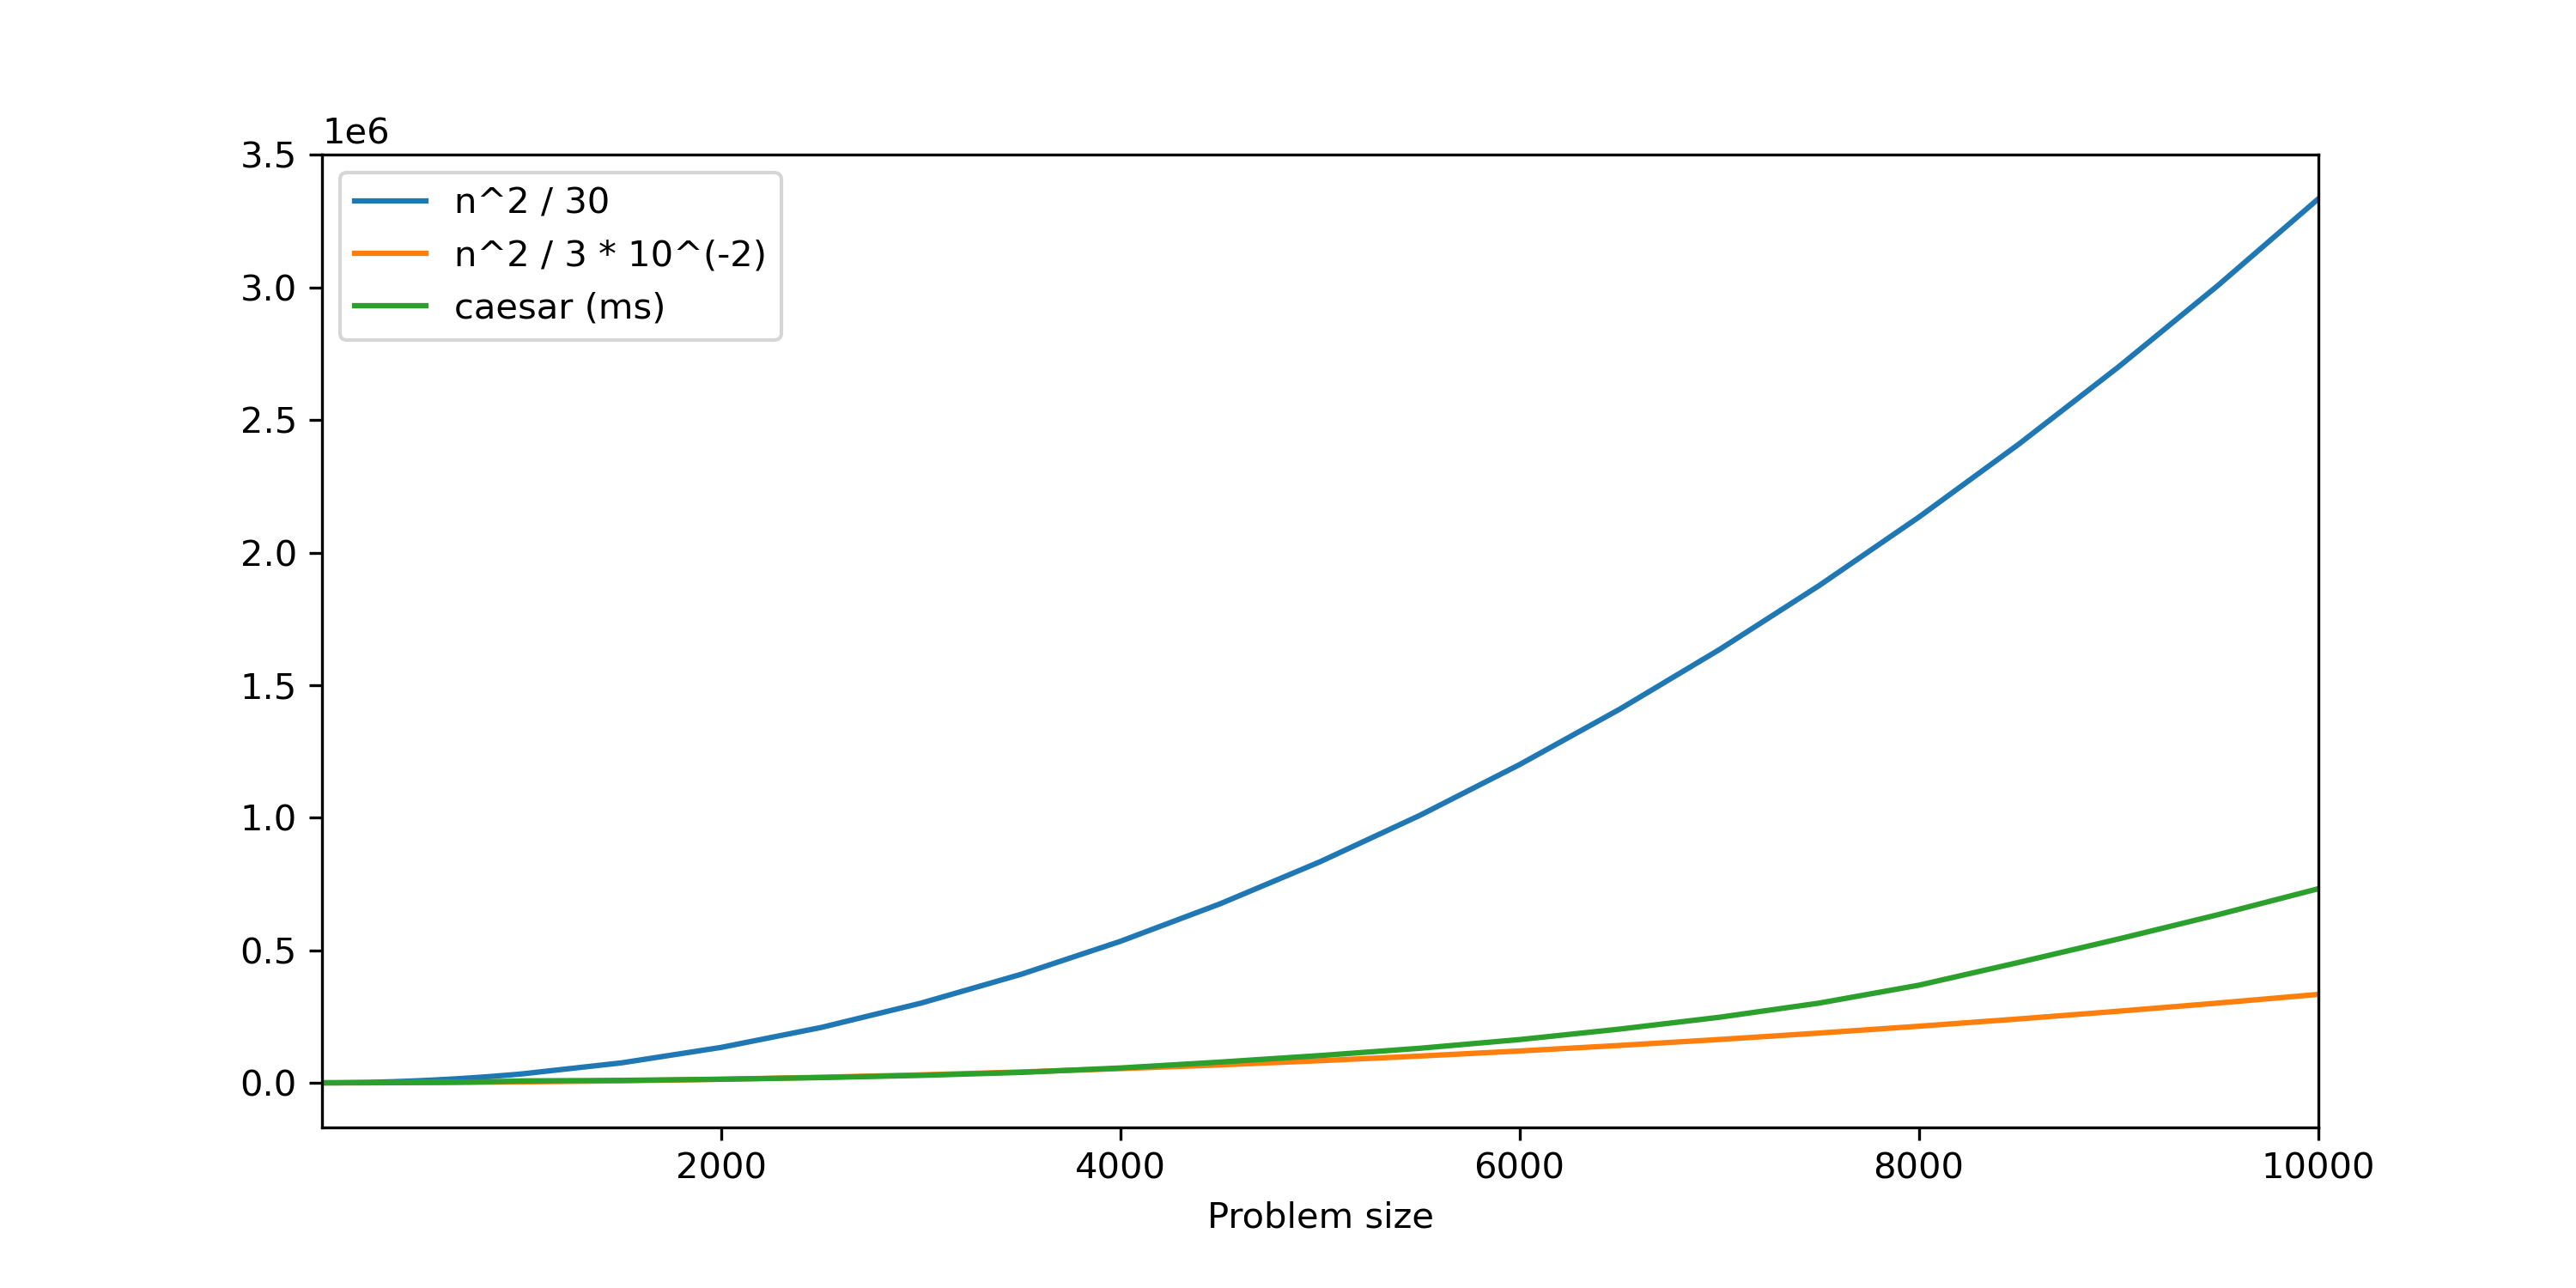
\includegraphics[width=1\textwidth]{O_caesar}
\end{figure}

These graphs allow us to say that our initial hypotheses about time complexities of the given algorithms indeed hold (at least for the ranges examined in this article), as the curves are squezeed between $x^2$  or  $x^{\log_2 3}$ with some coefficents that are displayed in the graphs.

\section{Conclusion and optimisations}

\subsection{Possible optimisation}
As it was previously mentioned, for big numbers \textbf{Divide and Conquer} algorithm fails to be effective(in terms of constant multiplier of complexity, not asymptotical values), however this can be improved by changing scheme: `divide numbers into equal parts` $\to$ `compute their products` $\to$  `sum up the results` to `if numbers are small` $\to$ `compute their product`; `else` $\to$ `do the previous scheme`. This logic can also be applied to the Karatsuba algorithm also and in theory make them work faster. In the graph below it can be seen that \textbf{Divide and Conquer} actually appears to be viable, while \textbf{Karatsuba} algorithm works faster than \textbf{School-grade} on the whole range from 1-digit numbers to 20000-digit numbers.  
\begin{figure}[h]
\caption{Algorithms with fallback from 16 digits}

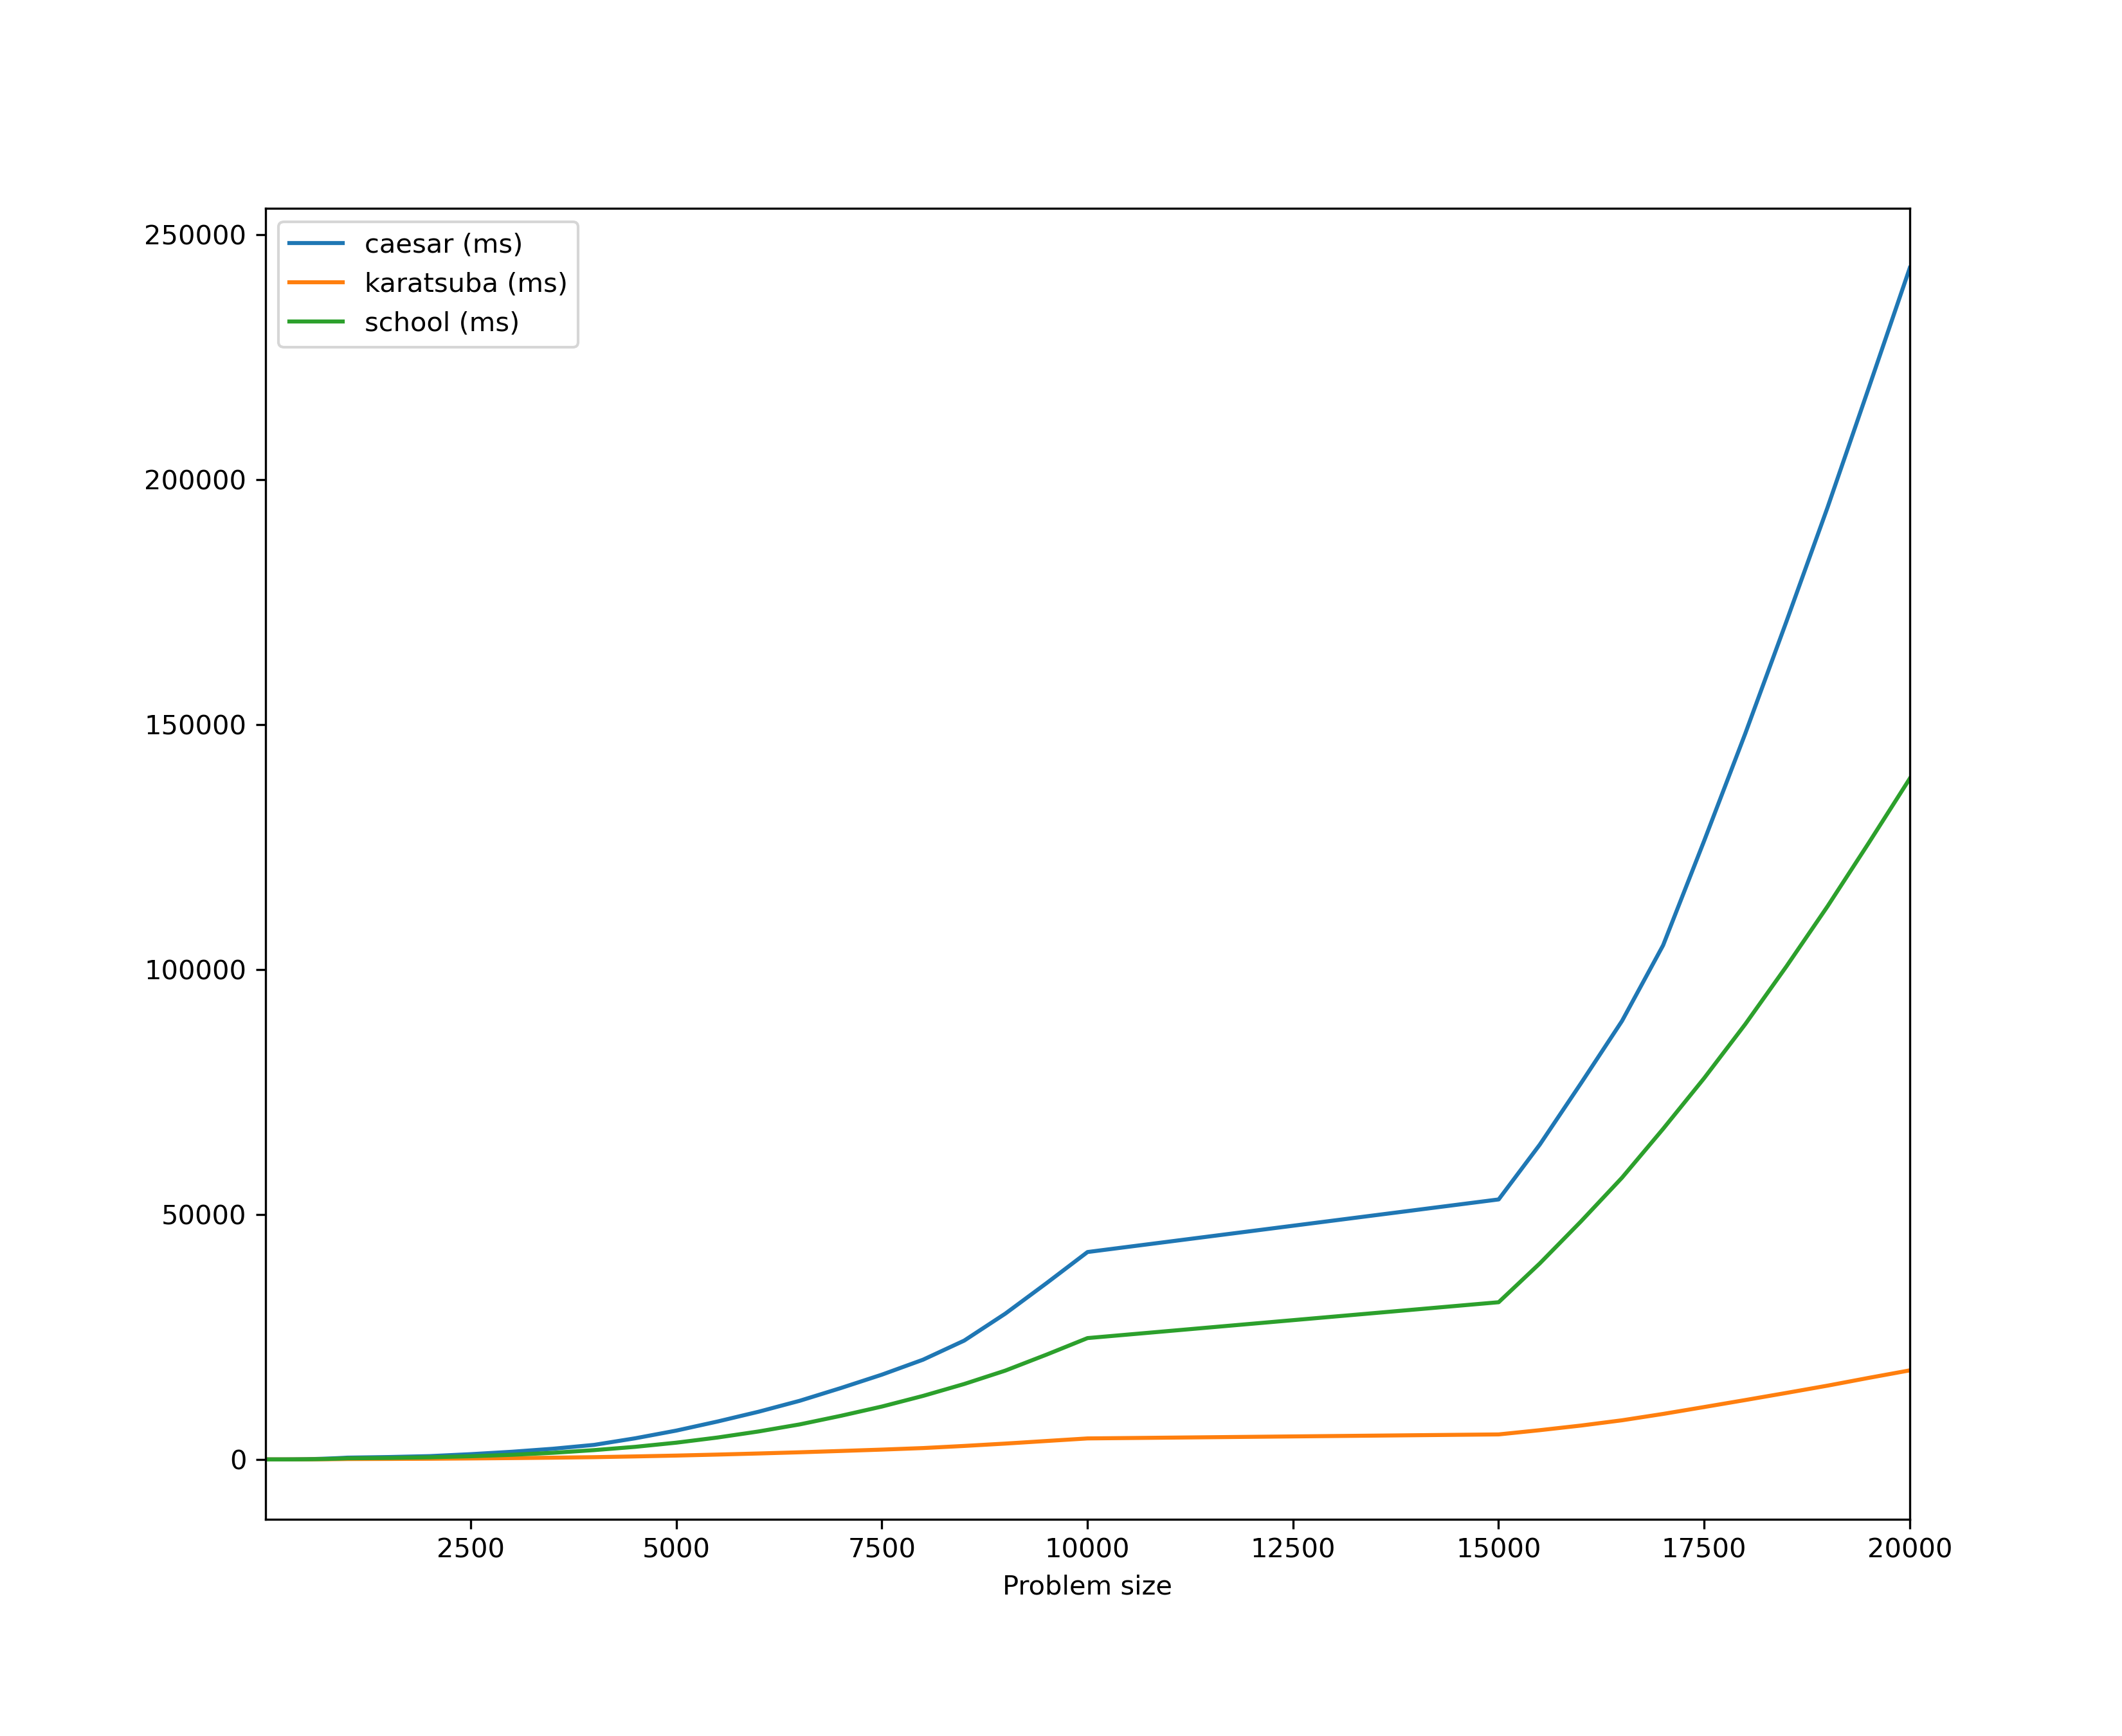
\includegraphics[width=1\textwidth]{optimised}
\end{figure}
\clearpage
\subsection{Conclusion}
What this article has established:
\begin{itemize}
\item  \textbf{Divide and Conquer} multiplication:
	$T(n) \in \Theta(n^2)$
\item  \textbf{School-grade} multiplication:
	$T(n) \in \Theta(n^2)$
\item  \textbf{Karatsuba} multiplication:
	$T(n) \in \Theta(n^{\log_2 3})$, works faster for $n>90000$, when not optimised.
\end{itemize}
In the end, it is possible to make all algorithms work better, for instance, now class `Number` is based on std::string and its notions, however starting from C++17 \ std::string\_view was introduced that would probably allow Number::operator+= and Number::split work faster significantly. Other direction of improvement may be to run all algorithms not 3 times to reduce error but more, for example 10, as well as to choose a wider range of problem sizes and make measurements more frequently. 
\end{document}